In diesem Abschnitt wird die Auswirkung unterschiedlicher Größen des Target-Datensatzes auf die Performanz der Netzwerke untersucht. Es wird 
die Hypothese überprüft, dass die Leistung mit abnehmender Datenmenge schlechter wird.

Für eine vergleichbare Basis werden alle Netzwerke jeweils über insgesamt 40 Epochen trainiert, wobei nach 20 Epochen ein TF 
durchgeführt wird. Diese Untersuchung erfolgt anhand der Netzwerke CMP, 1DC und COD. Zusätzlich wird auch die Performanz auf dem Testdatensatz 
betrachtet.

\begin{figure}[htpb]
    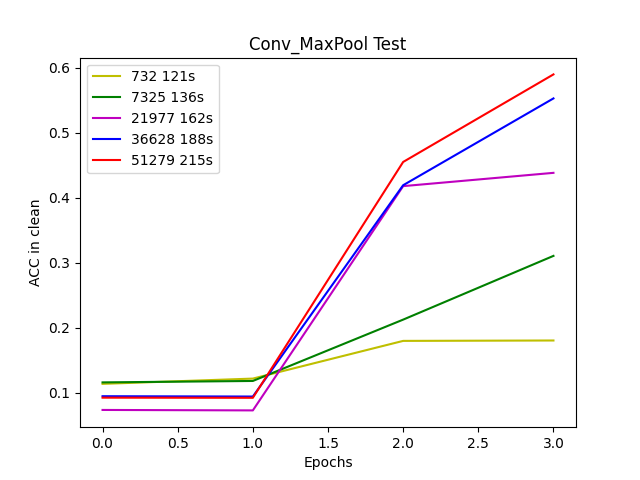
\includegraphics[height=5cm]{../../Plots/ba_plots/targetgroesse/cmp_ts.png}
    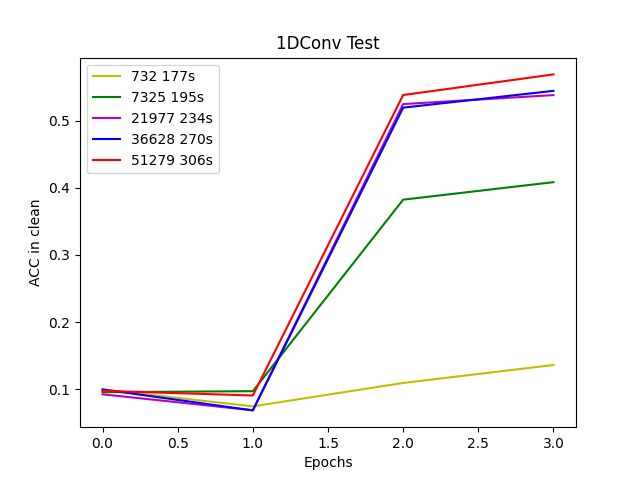
\includegraphics[height=5cm]{../../Plots/ba_plots/targetgroesse/1dc_ts.png}
    \caption{\label{fig:targetgroessedeepdir} 
    \small{Abgebildet ist die Veränderung der Accuracy bei Convolutional-Netzwerken in Abhängigkeit von der Größe des Target-Datensatzes. Die 
    Plots zeigen jeweils die Ergebnisse auf dem Testdatensatz des Target-Datensatzes, wobei links das CMP-Netzwerk und rechts das 1DC-Netzwerk 
    dargestellt sind.
    Die dargestellten Tests umfassen für CMP die Varianten CMP:TF2/732/10, CMP:TF2/7k/10, CMP:TF2/21k/10, CMP:TF2/36k/10 und CMP:TF2/51k/10, 
    sowie für 1DC die Varianten 1DC:TF2/732/10, 1DC:TF2/7k/10, 1DC:TF2/21k/10, 1DC:TF2/36k/10 und 1DC:TF2/51k/10, jeweils dargestellt in den 
    Farben Gelb, Grün, Lila, Blau und Rot.
    }}
\end{figure}

In Abbildung \ref{fig:targetgroessedeepdir} sind die Testläufe in Abhängigkeit von der Größe des Trai-\\ningsdatensatzes dargestellt. Die erste 
Zahl in der Legende bezeichnet die Datenmenge, die zweite Zahl die Trainingsdauer. Die Datenmenge bezieht sich ausschließlich auf den 
Target-Datensatz. Es zeigt sich, dass die Trainingsdauer mit zunehmender Datenmenge ansteigt. Zudem bestätigt sich die Annahme, dass die 
Performanz bei Kaskadennetzwerken mit TF mit wachsender Datenmenge verbessert wird. Darüber hinaus weist das Deep Cascade 
Netzwerk eine leicht bessere Performanz auf als das Direct Cascade Netzwerk, was vermutlich darauf zurückzuführen ist, dass Direct Cascade 
Netzwerke lediglich ein Hidden Layer besitzen, während Deep Cascade Netzwerke aus mehreren Hidden Layern bestehen und daher in der Lage sind, 
komplexere Problemstellungen effizienter zu erlernen. 

\begin{figure}[htpb]
    \centering
    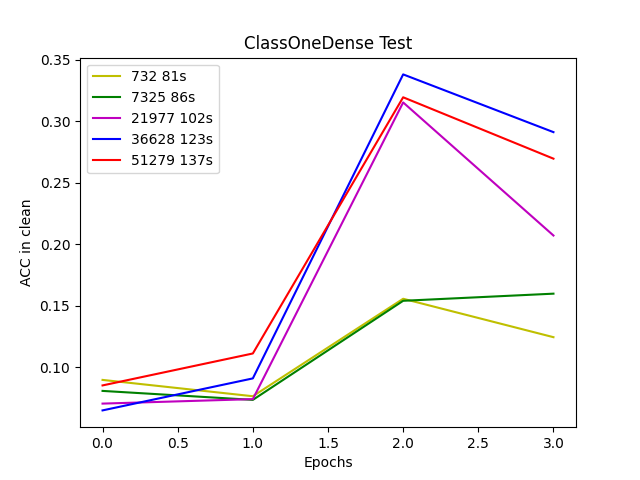
\includegraphics[height=5cm]{../../Plots/ba_plots/targetgroesse/cod_ts.png}
    \caption{\label{fig:targetgroesselinear} 
    \small{Abgebildet ist die Veränderung der Test-Accuracy eines linearen Netz-werks in Abhängigkeit von der Größe des Target-Datensatzes. 
    Die dargestellten Tests umfassen die Varianten COD:TF2/732/10, COD:TF2/7k/10, COD:TF2/21k/10, COD:TF2/36k/10 und COD:TF2/51k/10, 
    dargestellt in den Farben Gelb, Grün, Lila, Blau und Rot.}}
\end{figure}

Abbildung \ref{fig:targetgroesselinear} zeigt die Ergebnisse des Direct Cascade Netzwerks, das aus-schließlich lineare Hidden Layer verwendet. 
Auffällig ist, dass dieses Netzwerk unabhängig von der Anzahl der Trainingsdaten stets eine schlechtere Performanz aufweist als die beiden 
anderen Netzwerke, welche Convolutional Layer enthalten. Dies ist darauf zurückzuführen, dass das lineare Netzwerk die relevanten Merkmale für 
die Bilderkennung nicht adäquat extrahieren kann, da die Daten eine komplexe und nicht-lineare Struktur aufweisen.

Generell zeigt sich in allen Testplots, dass die erzielte Accuracy der Netz-werke mit TF selbst bei ausreichender Datenmenge, die ein direktes 
Training auf dem 
Target-Datensatz ermöglichen würde, nie eine zufriedenstellend hohe Accuracy erreicht. Das direkte Training auf dem Target-Datensatz mit dem 
Deep Cascade Netzwerk mit sehr vielen Trainingsbeispielen hingegen erzielt eine Accuracy von etwa 70\%, was deutlich über den Ergebnissen der 
TF Netzwerke liegt.
